\documentclass{article}
\usepackage{xcolor}
\newcommand{\red}{\color{red}}
\usepackage{tikz}
\usepackage[width=200mm]{geometry}
\pagestyle{empty}

\begin{document}

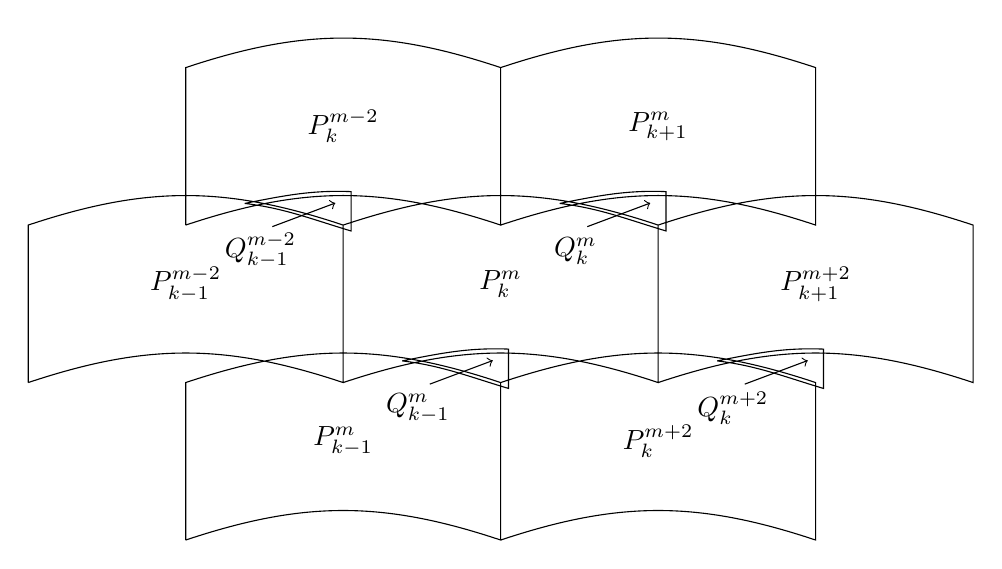
\begin{tikzpicture}
	%\draw[help lines] (-1,-1) grid (12,6);
	\draw
	%% P

	% m-2
	(0,0) .. controls +(1.5,.5) and +(-1.5,.5) .. ++(4,0)
	-- ++(0,2) .. controls +(-1.5,.5) and +(1.5,.5) .. ++(-4,0)
	-- ++(0,-2) +(2,1.25) node{$P_{k-1}^{m-2}$}

	(2,2) .. controls +(1.5,.5) and +(-1.5,.5) .. ++(4,0)
	-- ++(0,2) .. controls +(-1.5,.5) and +(1.5,.5) .. ++(-4,0)
	-- ++(0,-2,0) +(2,1.25) node{$P_{k}^{m-2}$}

	% m
	(2,-2) .. controls +(1.5,.5) and +(-1.5,.5) .. ++(4,0)
	-- ++(0,2) .. controls +(-1.5,.5) and +(1.5,.5) .. ++(-4,0)
	-- ++(0,-2,0) +(2,1.25) node{$P_{k-1}^{m}$}

	(4,0) .. controls +(1.5,.5) and +(-1.5,.5) .. ++(4,0)
	-- ++(0,2) .. controls +(-1.5,.5) and +(1.5,.5) .. ++(-4,0)
	-- ++(0,-2,0) +(2,1.25) node{$P_{k}^{m}$}

	(6,2) .. controls +(1.5,.5) and +(-1.5,.5) .. ++(4,0)
	-- ++(0,2) .. controls +(-1.5,.5) and +(1.5,.5) .. ++(-4,0)
	-- ++(0,-2,0) +(2,1.25) node{$P_{k+1}^{m}$}

	% m+2
	(6,-2) .. controls +(1.5,.5) and +(-1.5,.5) .. ++(4,0)
	-- ++(0,2) .. controls +(-1.5,.5) and +(1.5,.5) .. ++(-4,0)
	-- ++(0,-2,0) +(2,1.25) node{$P_{k}^{m+2}$}

	(8,0) .. controls +(1.5,.5) and +(-1.5,.5) .. ++(4,0)
	-- ++(0,2) .. controls +(-1.5,.5) and +(1.5,.5) .. ++(-4,0)
	-- ++(0,-2,0) +(2,1.25) node{$P_{k+1}^{m+2}$}

	%%Q

	% m-2
	(2.75,2.275) .. controls +(.5,.1) and +(-.5,.02) .. ++(1.35,0.15)
	-- ++(0,-.5) .. controls +(-.5,.15) and +(.5,-.06) .. ++(-1.35,.35)
	+(.2,-.6) node{$Q_{k-1}^{m-2}$}

	% m
	(6.75,2.275) .. controls +(.5,.1) and +(-.5,.02) .. ++(1.35,0.15)
	-- ++(0,-.5) .. controls +(-.5,.15) and +(.5,-.06) .. ++(-1.35,.35)
	+(.2,-.6) node{$Q_{k}^{m}$}

	(4.75,0.275) .. controls +(.5,.1) and +(-.5,.02) .. ++(1.35,0.15)
	-- ++(0,-.5) .. controls +(-.5,.15) and +(.5,-.06) .. ++(-1.35,.35)
	+(.2,-.6) node{$Q_{k-1}^{m}$}

	% m+2
	(8.75,0.275) .. controls +(.5,.1) and +(-.5,.02) .. ++(1.35,0.15)
	-- ++(0,-.5) .. controls +(-.5,.15) and +(.5,-.06) .. ++(-1.35,.35)
	+(.2,-.6) node{$Q_{k}^{m+2}$}

	;

	% m-2 
	\draw[->] (2.9,2.28) ++(.2,-.3) -- ++(.8,.3);
	% m
	\draw[->] (6.9,2.28) ++(.2,-.3) -- ++(.8,.3);
	\draw[->] (4.9,0.28) ++(.2,-.3) -- ++(.8,.3);
	% m+2
	\draw[->] (8.9,0.28) ++(.2,-.3) -- ++(.8,.3);

	;

\end{tikzpicture}

\end{document}
